\section{32-bit substraction}
\subsection{Aim}
To substract two 32-bit numbers

\subsection{Code}
\begin{lstlisting}
DATA SEGMENT
	subtrahend DD 1000H
	minuend DD 500H
	difference DD ?
ENDS DATA

CODE SEGMENT
ASSUME CS:CODE, DS:DATA
START:
	MOV AX, DATA
	MOV DS, AX
	MOV AX, [subtrahend]
	MOV BX, [minuend]
	SUB AX, BX
	MOV [difference], AX
	MOV AX, [subtrahend+2]
	MOV BX, [minuend+2]
	SUB AX, BX
	MOV [difference+2], AX
	MOV AH, 04CH
    INT 21H
ENDS CODE
END START
\end{lstlisting}

\subsection{Output}
\begin{center}
	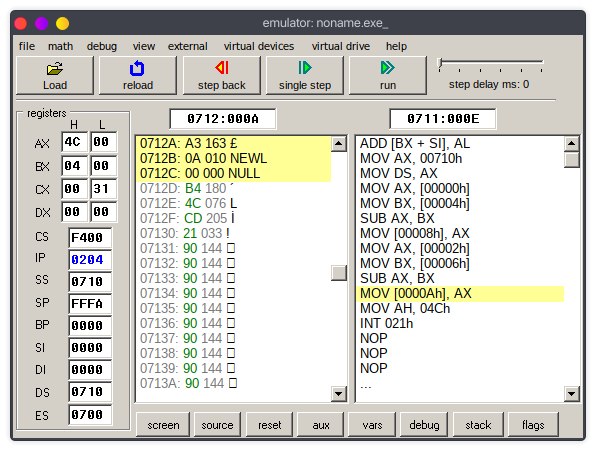
\includegraphics[width=0.90\textwidth]{img/p4/ss1.png}
	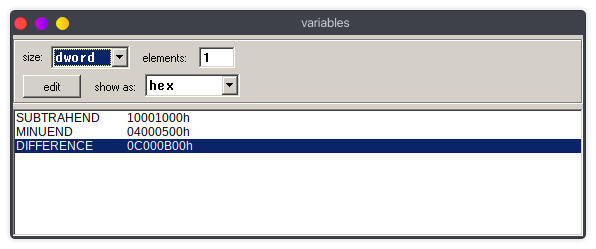
\includegraphics[width=0.90\textwidth]{img/p4/ss2.png}
\end{center}

\subsection{Result}
Two 32 bit numbers were substracted in emu8086 and output was verified